\section{PART 2: Exit the Monad, Enter the Handler}
\begin{frame}
  \frametitle{Algebraic effects}
  \begin{columns}
    \begin{column}{0.5\textwidth}
      \begin{center}
        \begin{figure}
          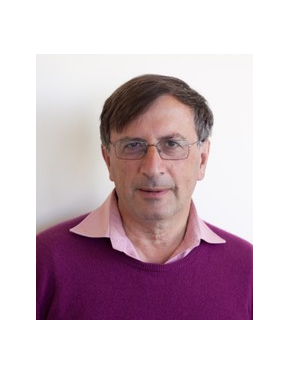
\includegraphics[scale=0.3]{figures/gordonplotkin.png}
          \caption{Gordon Plotkin}
        \end{figure}
      \end{center}
    \end{column}
    \begin{column}{0.5\textwidth}
      \begin{center}
        \begin{figure}
          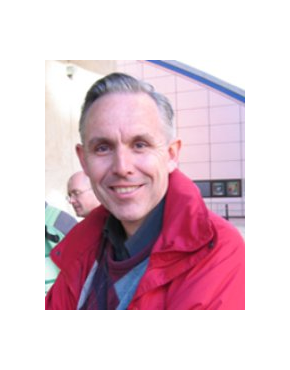
\includegraphics[scale=0.3]{figures/johnpower.png}
          \caption{John Power}
        \end{figure}
      \end{center}
    \end{column}
  \end{columns}
\end{frame}

\begin{frame}
  \frametitle{Algebraic effects and computations}
  \begin{definition}{Algebraic effect}
    An algebraic effect is a collection of abstract operations, e.g. 
    $\{ Op_i : a_i \to b_i \}$
  \end{definition}
  \begin{definition}{Abstract computation}
    An abstract computation is composed from abstract operations. Computations have type
    %$() \xrightarrow{\{Op_i : a_i \to b_i \; | \; \rho\}\;} c$
  \end{definition}

%   \begin{block}{Handler}
%     A handler interprets an abstract computation $m$.
% \begin{lstlisting}[basicstyle=\small\ttfamily]
% (*\only<2-2>{\texttt{open }}*)handler(m) {
%   case Op(*$_i$*)(p(*$_i$*),k(*$_i$*))  (*$\to$*) body(*$_i$*)
%   case Return(x)  (*$\to$*) x
% }
% \end{lstlisting}
% Typing: \only<1-1>{$(() \xrightarrow{\{Op_i : a_i \to b_i\}\;} c) \to d$}\only<2-2>{$(() \xrightarrow{\{Op_i : a_i \to b_i \; | \; \rho\}\;} c) \to () \xrightarrow{\{Op_i:\alpha \; | \; \rho\}} \to d$}
%   \end{block}
\end{frame}

% \begin{frame}[fragile]
%   \frametitle{Effects as computation trees \cite{Lindley14}}
% Operation $\textsf{Choose} : () \to \texttt{Bool}$.

% \vspace{0.5cm}
% Picture the CPS term $\textsf{Choose}_{()}(\textsf{Choose}_{()}(2,4),\textsf{Choose}_{()}(8,16))$, e.g.
% \vspace{0.5cm}
% \begin{center}
% \begin{tikzpicture}[level distance=1.5cm,
% level 1/.style={sibling distance=3.5cm},
% level 2/.style={sibling distance=1cm}]
% %\tikzstyle{every node}=[circle,draw]

% \node (Root) [blue,rectangle] {Choose ()}
%     child { node[blue] (q0) {Choose ()} 
%       child { node[draw=none] (q00) {2}
%       }
%       child { node[draw=none] (q01) {4} 
%       }
%       edge from parent node [draw=none,left,xshift=-2.0,yshift=2.0] {true}
%     }
%     child { node [blue] (q1) {Choose ()}
%       child { node[draw=none] (q10) {8}
%       }
%       child { node[draw=none] (q11) {16}       
%       }
%       edge from parent node [draw=none,right,xshift=2.0,yshift=2.0] {false}
%     };

% \only<2-2>{\draw[->,red,rounded corners,dashed,line width=0.7pt]
%     ($(Root) +(-1.0,0.2)$) --
%     ($(q0) +(-1.0,0.4)$) --
%     ($(q00) +(-0.3,0.0)$);}

% \only<3-3>{\draw[->,red,rounded corners,dashed,line width=0.7pt]
%     ($(Root) +(1.0,0.2)$) --
%     ($(q1) +(1.0,0.4)$) --
%     ($(q10) +(1.3,0.0)$);}

% \only<4-5>{\draw[->,red,rounded corners,dashed,line width=0.7pt]
%     ($(Root) +(-1.0,0.2)$) --
%     ($(q0) +(-1.0,0.4)$) --
%     ($(q00)  +(-0.5,0.0)$) --
%     ($(q00)  +(-0.4,-0.35)$) --
%     ($(q00)  +(0.0,-0.5)$) --
%     ($(q00)  +(0.4,-0.35)$) --
%     ($(q00)  +(0.5,0.0)$) --
%     ($(q0)  +(-0.005,-0.3)$) --
%     ($(q01)  +(-0.35,-0.35)$) --
%     ($(q01)  +(0.0,-0.45)$) --
%     ($(q01)  +(0.35,-0.35)$) --
%     ($(q01)  +(0.4,0.0)$) --
%     ($(q0)   +(1.0,0.5)$) --
%     ($(Root) +(-0.3,-0.4)$) --
%     ($(q1)  +(-0.8,-0.1)$) --
%     ($(q10)  +(-0.5,0.0)$) --
%     ($(q10)  +(-0.4,-0.35)$) --
%     ($(q10)  +(0.0,-0.5)$) --
%     ($(q10)  +(0.4,-0.35)$) --
%     ($(q10)  +(0.5,0.0)$) --
%     ($(q1)  +(-0.005,-0.3)$) --
%     ($(q11)  +(-0.35,-0.35)$) --
%     ($(q11)  +(0.0,-0.45)$) --
%     ($(q11)  +(0.35,-0.35)$) --
%     ($(q11)  +(0.4,0.0)$);}
% \end{tikzpicture}
% \end{center}
% \only<1-1>{How should we interpret this computation?}
% \only<2-2>{$\Rightarrow$ $2 : \texttt{Int}$ (Strictly positive)}
% \only<3-3>{$\Rightarrow$ $16 : \texttt{Int}$ (depressingly pessimistic)}
% \only<4-4>{How about this?}
% \only<5-5>{$\Rightarrow [2,4,8,16] : [\texttt{Int}]$}
% \end{frame}

\begin{frame}
  \frametitle{Nim: A game with sticks}
  \begin{center}
    \begin{figure}
      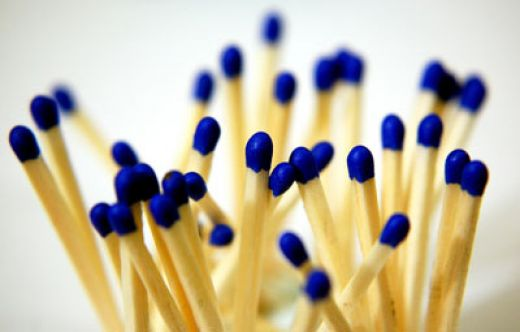
\includegraphics[scale=0.3]{sticks.jpg}
    \end{figure}
  \end{center}
  Set-up
  \begin{itemize}
    \item Two players: Alice and Bob; Alice always starts.
    \item One heap of $n$ sticks.
    \item Turn-based. Each player take between 1-3 sticks.
    \item The one, who takes the last stick, wins.
  \end{itemize}
We'll demonstrate how to encode strategic behaviour, compute game data, and cheat using handlers.
\end{frame}

\begin{frame}
  \frametitle{Game tree generated by \texttt{mtGen} with $n = 3$}
\begin{center}
\begin{tikzpicture}[level distance=1.5cm,
level 1/.style={sibling distance=3.5cm},
level 2/.style={sibling distance=2cm}]
%\tikzstyle{every node}=[circle,draw]

\node (Root) [blue,rectangle] {Alice}
    child { node[red] (q0) {Bob} 
      child { node[blue] {Alice}
        child { node[draw=none] {Alice wins}
          edge from parent node [draw=none,left,xshift=-2.3,yshift=2.3] {1}
        }
        edge from parent node [draw=none,left,xshift=-2.0,yshift=2.0] {1}
      }
      child { node[draw=none] {Bob wins}
        edge from parent node [draw=none,right,xshift=2.0,yshift=2.0] {2}
      }
      edge from parent node [draw=none,left,xshift=-2.0,yshift=2.0] {1}
    }
    child { node [red] {Bob}
      child { node[draw=none] {Bob wins}
        edge from parent node [draw=none,right,xshift=2.0,yshift=2.0] {1}
      }
    }
    child { node [draw=none] {Alice wins}
      edge from parent node [draw=none,right,xshift=2.0,yshift=2.0] {3}
    };    
\end{tikzpicture}
%Take((Alice(), [(1, Take((Bob(), [(1, Take((Alice(), [(1, Winner(Alice()))]))),
%#                                    (2, Winner(Bob()))]))),
%#                  (2, Take((Bob(), [(1, Winner(Bob()))]))),
%#     		   (3, Winner(Alice()))]))
\end{center}
\end{frame}

% \begin{frame}[fragile]
%   \frametitle{Concrete syntax}
%   \begin{block}{Handlers}
%     Essentially, handlers embody a collection of case-statements, e.g.
% \begin{lstlisting}[basicstyle=\ttfamily]
% handler(m) {
%   case Op1(p,k)  -> ...
%   case OpN(p,k)  -> ...
%   case Return(x) -> ...
% } 
% \end{lstlisting}
% This style is adapted from Plotkin and Pretnar \cite{Plotkin13,Kammar13}.
%   \end{block}
%   \begin{block}{Operation discharge}
%     Operations are discharged using the ``do'' primitive, e.g.
%     \texttt{do Op(arg)}
%   \end{block}
% \end{frame}

% \begin{frame}
%   \frametitle{How does row polymorphism fit into this?}
%   \begin{itemize}
%     \item Handlers get typed as
%   \[ \texttt{fun} : (() \xrightarrow{\{Op_1:a_1 \to b_1,\dots,Op_n:a_n \to b_n \}\;} c) \to c \]
%   that is, they are closed.\\
% \item \uncover<2->{We want \emph{open} handlers too, e.g.}
%   \uncover<2->{\[ \texttt{fun} : (() \xrightarrow{\{Op_1:a_1 \to b_1,\dots,Op_n:a_n \to b_n \; | \; \rho \}\;} c) \to c \]
% Consequently, we obtain a high-degree of modularity.
% }

% \end{itemize}
% \end{frame}